% \iffalse meta-comment
%
%% File: bearwear.dtx
%
% Copyright (C) 2020 Ulrike Fischer / Bär
%
% It may be distributed and/or modified under the conditions of the
% LaTeX Project Public License (LPPL), either version 1.3c of this
% license or (at your option) any later version.  The latest version
% of this license is in the file
%
%    https://www.latex-project.org/lppl.txt
%
% This file is part of the "bearwear bundle" (The Work in LPPL)
% and all files in that bundle must be distributed together.
%
% -----------------------------------------------------------------------
%
% The development version of the bundle can be found at
%
%    https://github.com/u-fischer/bearwear
%
% for those people who are interested.
%
%<*driver>
\documentclass{l3doc}
\OnlyDescription
\PassOptionsToPackage{svgnames}{xcolor}
\usepackage{tikzlings,tikzducks,bearwear}
\usetikzlibrary{patterns,patterns.meta}
\usepackage{csquotes,graphicx}
\usepackage{needspace}
\usepackage{AlegreyaSans}
\setmainfont{Heuristica}
\usepackage[most]{tcolorbox}

\lstdefinestyle{bearwarestyle}{% stolen and adapted from tikzlings
	language={[latex]TeX},
	tabsize=2,
	breaklines,
	basicstyle=\ttfamily,
	commentstyle={\color{green!50!black}\slshape},
	columns=fullflexible,
	alsodigit={-},
	alsoletter={3},
	emphstyle=\color{red!60!black},
	emph=[1]{
		v-neckline,muscle, shirt, t-shirt, long, sleeves, round, neckline,
        leftarm, rightarm,arms,deco,body, pattern,beartummy,
        bearheart,color},
	texcsstyle=*\color{SteelBlue!50!black}\bfseries,
	keywordstyle=\color{red!60!black}\bfseries,
	morekeywords={tikzpicture},
	moretexcs={bearwear, bearwearsetup},
	delim ={[s][\ttfamily\color{green!50!black}]{$}{$}},
	moredelim=[is][\footnotesize\ttfamily\color{orange!70!black}]{|}{|},
	index=[1][emph]
}
\tcbset{%
	colframe=SteelBlue!50!black,
	arc=0mm,
	fonttitle=\bfseries,
	sidebyside,
	listing options={style=bearwarestyle},
	center lower,
	righthand width=4cm,
	bottom=0pt,
	top=0pt,
	%tikz lower,
	height plus=3cm,
	colback=SteelBlue!30!white,
    enlarge top initially by=10pt
}
\lstset{style=bearwarestyle}
\tikzset{
  hippo/.pic = {
   \begin{scope}[scale=0.2,transform shape]
     \hippo;
      \begin{scope}[yshift=0.15cm,xshift=-0.5cm,rotate=8]
        \duck[invisible,bowtie]
      \end{scope}
  \end{scope}},}
\raggedbottom
\let\bearwearkey\lstinline
\newcommand{\TikZ}{Ti\emph{k}Z}

\GetFileInfo{bearwear.sty}
\title{The \bearwearlogo{} Package%
       \thanks{This file describes \fileversion,
        last revised \filedate.}}
\author{Idea: Bär~~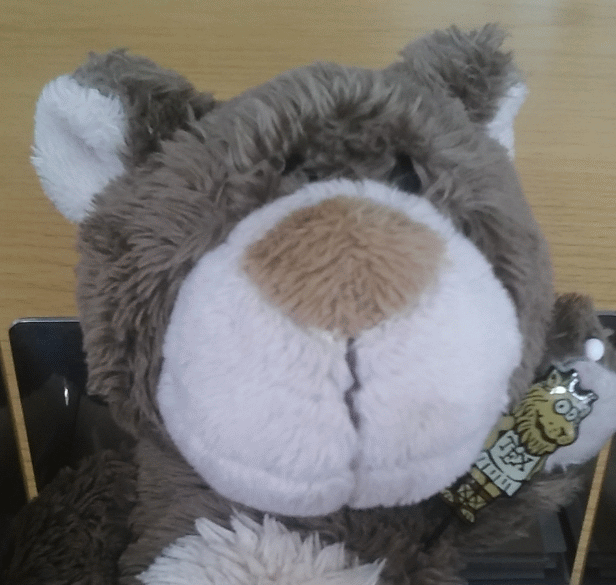
\includegraphics[trim=0pt 15pt 0pt 0pt,height=13pt]{baer}
        \and Implementation: Ulrike Fischer%
        \thanks{Issues should be reported at https://github.com/u-fischer/bearwear}
        ~
\includegraphics[trim=0pt 15pt 0pt 0pt,height=15pt]{ulrike}}
\date{\filedate}
\begin{document}
  \DocInput{\jobname.dtx}
\end{document}
%</driver>
% \fi
% \maketitle
% \section{Basic Usage}
\subsection{The shirts}
 The package provides a number of shirts for the bear, \bearwearkey{long sleeves} and \bearwearkey{round neckline} are the defaults:
 \begin{tcblisting}{} 
 \tikz\bearwear % default values
    [long sleeves, round neckline];
 \tikz\bearwear
   [t-shirt];
 \tikz\bearwear
   [muscle shirt];
 \tikz\bearwear
   [v-neckline];
 \tikz\bearwear
   [t-shirt,v-neckline];
 \tikz\bearwear
   [muscle shirt,v-neckline];
  \end{tcblisting}
  
 \subsection{Dressing the bear}
 
 To dress the shirt with the bear, simply add the \verb+\bear+ command from the \bearwearkey{tikzlings-bears} package.
 
 \begin{tcblisting}{}
 \tikz{\bear;\bearwear[v-neckline];}
 \tikz{\bear;\bearwear[muscle shirt];}
  \end{tcblisting}
  
 \subsection{Coloring the shirts}

 The body and the arms of the shirts can be colored:

 \begin{tcblisting}{}
 \tikz{\bear;
       \bearwear
       [v-neckline,
       leftarm=red,body=blue,rightarm=green];}
 \tikz{\bear;\bearwear[arms=green];}
 \tikz{\bear;
       \bearwear
         [shirt=
           {shade,
            top color=blue, 
            bottom color=red}];}
 \end{tcblisting} 
 
 The keys \bearwearkey{arms} and \bearwearkey{shirt} are meta keys which execute the three basic keys \bearwearkey{leftarm}, \bearwearkey{rightarm} and \bearwearkey{body}.
 
 Basically everything that would make sense in a \verb+\fill+ option is allowed here.  Patterns e.g. would work too:
 
 \begin{tcblisting}{}
 \tikz{\bear;
       \bearwear
       [v-neckline,
        shirt  =
         {pattern=
          horizontal lines light blue}];}
 \end{tcblisting} 
 
 
 \subsection{Additional patterns}
 
 As seen in the last example patterns can be added with the previous keys, but sometimes it makes sense to add them on top to preserve a background color. For this the package provides special \texttt{pattern} keys: 
 \bearwearkey{leftarm pattern}, \bearwearkey{rightarm pattern}, \bearwearkey{arms pattern},
 \bearwearkey{body pattern}, \bearwearkey{shirt pattern},
 
 \begin{tcblisting}{}
 \tikz{\bear;
       \bearwear
       [v-neckline,
        shirt=red,
        body pattern = 
         {pattern=
          {Stars[points=6,radius=0.5mm,distance=1.5mm]},
         pattern color=yellow}];}
 \end{tcblisting} 
  
 
  
 \subsection{Decorations}
 
 The \texttt{deco} keys add their value to a \texttt{path picture} key. 
 
 \begin{tcblisting}{}
  \tikz{\bear;
  \bearwear[shirt deco = 
    {\node at (bearcenter) {
\includegraphics[width=5cm]{tartan3}};}]}
    
  \tikz{\bear;
   \bearwear[body deco=
    {\node at ([yshift=-1mm]bearchest) {
\includegraphics[width=0.3cm]{flag}};}];}  
    
  \tikz{\bear;
   \bearwear[shirt=Beige!80!black,
     body deco=
    {\node at ([yshift=-1mm]bearchest) {
\includegraphics[width=0.5cm]{latex-project-logo}};}];}     
  
  \tikz{\bear;
   \bearwear[shirt=HotPink,
     body deco=
    {\path  (bearchest)--++(0,-3mm)pic{hippo};}]}     
 \end{tcblisting}
 
  
%
% \StopEventually{}
%    \begin{macrocode}
%<@@=bearwear>
%<*package>
\RequirePackage{xparse}
\RequirePackage{tikzlings-bears}
\ProvidesExplPackage {bearwear} {2020-01-15} {0.1}
  {A package for tikz bear fashion}
\ProcessOptions\relax
% a tikzset style to reverse the clip:
\tikzset
  {@@reverseclip/.style=
    {insert~path=
      {
       (current~bounding~box.south~west) --  (current~bounding~box.north~west)
       --
       (current~bounding~box.north~east) --  (current~bounding~box.south~east)
       -- cycle
      }
   }
 }

\definecolor{@@europablue}{RGB}{00,33,99}

\cs_new_protected:Npn \@@_rightarm_path:nn #1 #2 %#1 fill, clip, #2 user
 {
  \path[#1,#2,rotate~around={-50\char_generate:nn{58}{12}(0.525,0.9)}]
    (0.525,0.9) ellipse (0.35~and~0.15);
 }

\cs_new_protected:Npn \@@_leftarm_path:nn #1 #2 %#1 fill, clip, #2 user
 {
   \path[#1,#2,rotate~around={50\char_generate:nn{58}{12}(-0.525,0.9)}]
     (-0.525,0.9) ellipse (0.35~and~0.15);
 }

\cs_new_protected:Npn \@@_body_path:nn #1 #2 %#1 fill, clip, #2 user
 {
   \path[#1,#2] (0,0.75) ellipse (0.55~and~0.65);
 }

\cs_new_protected:Npn \@@_init_path:
  {
    \@@_rightarm_path:nn {}{}
    \@@_leftarm_path:nn  {}{}
    \@@_body_path:nn     {}{}
  }

\cs_new_protected:Npn \@@_set_coordinates:
  {
    \coordinate (beartummy) at (0,0.75);
    \coordinate (bearheart)  at (0.25,0.9);
  }

\cs_new_protected:Npn \@@_clipping_path:
  {
    \bool_if:NTF  \l__bearwear_v_neckline_bool
     {
       \clip  (0, 1.55)     circle (0.5)    [__bearwearreverseclip]; %head
       \clip  (-0.4, 1.55) -- (0.4, 1.55) -- (0,0.8) --cycle[__bearwearreverseclip];
        %v-neck
     }
      {
       \clip  (0, 1.55)     circle (0.53)    [__bearwearreverseclip]; %head
     }
    \clip  (0.425, 0.3)  circle (0.28)   [@@reverseclip];
    \clip  (-0.425, 0.3) circle (0.28)   [@@reverseclip];
    \bool_if:NTF \l_@@_t_shirt_bool
     {
       \clip (-1,0.6) --++ (0.45,0)--++(-0.5,5) --cycle[@@reverseclip] ;
       \clip ( 1,0.6) --++ (-0.45,0)--++(0.5,5) --cycle[@@reverseclip] ;
     }
     {
       \clip (-1,0.6) --++ (0.45,0)--++(-0.5,1) --cycle[@@reverseclip] ;
       \clip ( 1,0.6) --++ (-0.45,0)--++(0.5,1) --cycle[@@reverseclip] ;
     }
    \clip(-1,0.5) rectangle (1,1.2);
  }

\cs_new_protected:Npn \@@_shirt_color:
  {
    \bool_if:NF \l_@@_muscle_shirt_bool
      {
        \exp_args:Nno \@@_leftarm_path:nn  {fill}{\l_@@_leftarm_color_tl}
        \exp_args:Nno \@@_rightarm_path:nn {fill}{\l_@@_rightarm_color_tl}
      }
    \exp_args:Nno \@@_body_path:nn     {fill}{\l_@@_body_color_tl}
  }

\cs_new_protected:Npn \@@_shirt_pattern:
  {
    \bool_if:NF \l_@@_muscle_shirt_bool
      {
        \exp_args:Nno \@@_leftarm_path:nn  {}{\l_@@_leftarm_pattern_tl}
        \exp_args:Nno \@@_rightarm_path:nn {}{\l_@@_rightarm_pattern_tl}
      }
    \exp_args:Nno \@@_body_path:nn         {}{\l_@@_body_pattern_tl}
  }

\cs_new_protected:Npn \@@_shirt_deco:
  {
    \bool_if:NF \l_@@_muscle_shirt_bool
      {
        \exp_args:Nno \@@_leftarm_path:nn  {}{\l_@@_leftarm_deco_tl}
        \exp_args:Nno \@@_rightarm_path:nn {}{\l_@@_rightarm_deco_tl}
      }
    \exp_args:Nno \@@_body_path:nn         {}{\l_@@_body_deco_tl}
  }

\bool_new:N \l_@@_t_shirt_bool
\bool_new:N \l_@@_muscle_shirt_bool
\bool_new:N \l__bearwear_round_neckline_bool

\tl_new:N \l_@@_leftarm_color_tl
\tl_new:N \l_@@_rightarm_color_tl
\tl_new:N \l_@@_body_color_tl

\tl_new:N \l_@@_leftarm_pattern_tl
\tl_new:N \l_@@_rightarm_pattern_tl
\tl_new:N \l_@@_body_pattern_tl
\tl_new:N \l_@@_leftarm_deco_tl
\tl_new:N \l_@@_rightarm_deco_tl
\tl_new:N \l_@@_body_deco_tl

\keys_define:nn {@@}
 {
   ,leftarm  .tl_set:N = \l_@@_leftarm_color_tl
   ,leftarm  .initial:n = {@@europablue}
   ,leftarm~pattern   .tl_set:N = \l_@@_leftarm_pattern_tl
   ,leftarm~deco         .code:n =
      {\tl_set:Nn \l_@@_leftarm_deco_tl {path~picture = {#1}}}
   ,rightarm .tl_set:N = \l_@@_rightarm_color_tl
   ,rightarm .initial:n = {@@europablue}
   ,rightarm~pattern   .tl_set:N = \l_@@_rightarm_pattern_tl
   ,rightarm~deco         .code:n =
      {\tl_set:Nn \l_@@_rightarm_deco_tl {path~picture = {#1}}}
   ,body     .tl_set:N = \l_@@_body_color_tl
   ,body     .initial:n = {@@europablue}
   ,body~pattern   .tl_set:N = \l_@@_body_pattern_tl
   ,arms     .meta:n   =  {leftarm={#1},rightarm={#1}}
   ,arms~pattern .meta:n   =  {leftarm~pattern={#1},rightarm~pattern={#1}}
   ,arms~deco .meta:n   =  {leftarm~deco={#1},rightarm~deco={#1}}
   ,shirt    .meta:n   =  {body={#1},leftarm={#1},rightarm={#1}}
   ,shirt~pattern    .meta:n   =
      {body~pattern={#1},leftarm~pattern={#1},rightarm~pattern={#1}}
   ,shirt~deco .meta:n   =
      {body~deco={#1},leftarm~deco={#1},rightarm~deco={#1}}
   ,long~sleeves .bool_set_inverse:N = \l_@@_t_shirt_bool
   ,t-shirt    .bool_set:N         = \l_@@_t_shirt_bool
   ,muscle~shirt .bool_set:N       = \l_@@_muscle_shirt_bool
   ,body~deco         .code:n =
      {\tl_set:Nn \l_@@_body_deco_tl {path~picture = {#1}}}
   ,round~neckline .bool_set_inverse:N       = \l__bearwear_v_neckline_bool
   ,v-neckline .bool_set:N   = \l__bearwear_v_neckline_bool
 }

\NewDocumentCommand\bearwearsetup { m }
 {
    \keys_set:nn { @@ } {#1}
 }
\NewDocumentCommand\bearwear { O {} }
  {
    \begin{scope}[even~odd~rule]
     % handle keys
     \keys_set:nn { @@ } {#1}
     \@@_init_path:
     \@@_set_coordinates:
     \@@_clipping_path:
     \@@_shirt_color:
     \@@_shirt_pattern:
     \@@_shirt_deco:
    \end{scope}
  }

\NewDocumentCommand\bearwearlogo {} {{
  \normalfont\fontencoding{T1}\fontfamily{AlegreyaSans-LF}\selectfont
   BearWear
   \raisebox{0.8ex}[0pt][0pt]{
     %\textcircled{
       \begin{tikzpicture}[baseline={(0,0.03)},scale=\fp_eval:n{\f@size/100}]
           \bear;
           \bearwear[body~deco={\node[text=white] at (beartummy)
              {\fontsize{\fp_eval:n{\f@size/20}pt}{\fp_eval:n{\f@size/20}pt}
                \sffamily
                BearWear};}]
       \end{tikzpicture}}}}%}
%</package>
%    \end{macrocode}
%<*docu>
 \section{Basic Usage}

 The package is based on \TikZ{} and the main command should be used in a \texttt{tikzpicture} or -- as shown in some of the examples -- with \verb+\tikz+.

 \subsection{The shirts}
 The package provides a number of shirts for the bear, \bearwearkey{long sleeves} and \bearwearkey{round neckline} are the defaults:
 \begin{tcblisting}{righthand width=6cm}
 \tikz\bearwear % default
    [long sleeves,
     round neckline];
 \tikz\bearwear
   [t-shirt];
 \tikz\bearwear
   [muscle shirt];

 \tikz\bearwear
   [v-neckline];
 \tikz\bearwear
   [t-shirt,v-neckline];
 \tikz\bearwear
   [muscle shirt,v-neckline];
  \end{tcblisting}

 \subsection{Dressing the bear}

 To dress the bear with the shirt, simply add the \verb+\bear+ command from the \bearwearkey{tikzlings-bears} package.

 \begin{tcblisting}{before=\nopagebreak}
 \tikz{\bear;\bearwear[v-neckline];}
 \tikz{\bear;\bearwear[muscle shirt];}
  \end{tcblisting}

 \subsection{Coloring the shirts}

 The body and the arms of the shirts can be colored. They are three basic keys: \bearwearkey{leftarm}, \bearwearkey{rightarm} and \bearwearkey{body}, and two meta keys: \bearwearkey{arms} and \bearwearkey{shirt}.

 \begin{tcblisting}{tikz lower}
  \bear;
  \bearwear
    [v-neckline,
     leftarm=red,
     rightarm=green,
     body=blue];
 \end{tcblisting}
 \begin{tcblisting}{tikz lower}
  \bear;
  \bearwear[arms=green];
 \end{tcblisting}
 \begin{tcblisting}{tikz lower}
  \bear;
  \bearwear
    [shirt=
      {shade,
       top color=blue,
       bottom color=red}];
 \end{tcblisting}


 Basically every option that would make sense in a \verb+\fill+  is allowed here.
 Patterns e.g. would work too:

 \begin{tcblisting}{tikz lower}
   \bear;
   \bearwear
     [v-neckline,
      shirt  =
        {pattern=
          horizontal lines light blue}];
 \end{tcblisting}


 \subsection{Additional patterns}

 As seen in the last example patterns can be added instead of colors, but sometimes it makes sense to
 add them on top to preserve a background color. For this the package provides special \texttt{pattern} keys:\\
 \bearwearkey{leftarm pattern}, \bearwearkey{rightarm pattern}, \bearwearkey{arms pattern},
 \bearwearkey{body pattern}, \bearwearkey{shirt pattern},

 \begin{tcblisting}{tikz lower}
  \bear;
  \bearwear
     [v-neckline,
      shirt=red,
      body pattern =
       {pattern=
         {Stars[points=6,
          radius=0.5mm,distance=1.5mm]},
        pattern color=yellow}];
 \end{tcblisting}



 \subsection{Decorations}

 The \lstinline|deco| keys add their value to a \texttt{path picture} key. This can be used to place emblems or use graphics as pattern. To help with the placement two coordinates are
 predefined: \bearwearkey{bearheart} and \bearwearkey{beartummy}.

 \begin{tcblisting}{tikz lower}
   \bear;
   \bearwear[shirt deco =
    {\fill[red] (beartummy) circle (1pt);
     \fill[red] (bearheart) circle (1pt);}
     ]
 \end{tcblisting}

 \begin{tcblisting}{tikz lower}
  \bear;
  \bearwear[shirt deco =
    {\node at (beartummy)
     {
\includegraphics[width=5cm]
       {tartan3}};}]
 \end{tcblisting}

 \begin{tcblisting}{tikz lower}
  \bear;
  \bearwear[body deco=
    {\node at ([yshift=-1mm]bearheart)
      {
\includegraphics[width=0.3cm]
        {flag}};}];
 \end{tcblisting}

 \begin{tcblisting}{tikz lower}
  \bear;
  \bearwear[
     shirt=Beige!80!black,
     body deco=
      {\node at ([yshift=-1mm]bearheart)
       {
\includegraphics[width=0.5cm]
         {latex-project-logo}};}];
 \end{tcblisting}

 \begin{tcblisting}{tikz lower}
  \bear;
  \bearwear[
     shirt=HotPink,
     body deco=
      {\path  (bearheart)--++(0,-3mm)
        pic{hippo};}];
 \end{tcblisting}


 \begin{tcblisting}{tikz lower}
  \bear;
  \bearwear[
    arms= DeepSkyBlue,
    body deco =
     {\node at ([yshift=-2mm]beartummy)
       {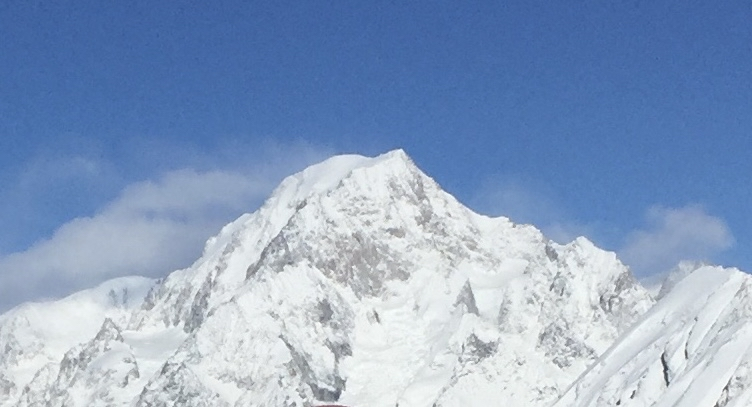
\includegraphics[width=4cm]
         {montblanc}};
      \node[text=white,
           font=\tiny\sffamily]
        at ([yshift=1.95mm]beartummy)
        {{Mont Blanc}};
     }]
 \end{tcblisting}

 \subsection{Scaling}

 Scaling works as expected, but don't forget that nodes in \TikZ{} normally don't scale if you don't use the \lstinline|transform shape| key:

 \begin{tcblisting}{tikz lower,before=\nopagebreak,}
  \begin{scope}[scale=1.5]
  \bear;
  \bearwear[
    arms= DeepSkyBlue,
    body deco =
     {\node at ([yshift=-2mm]beartummy)
       {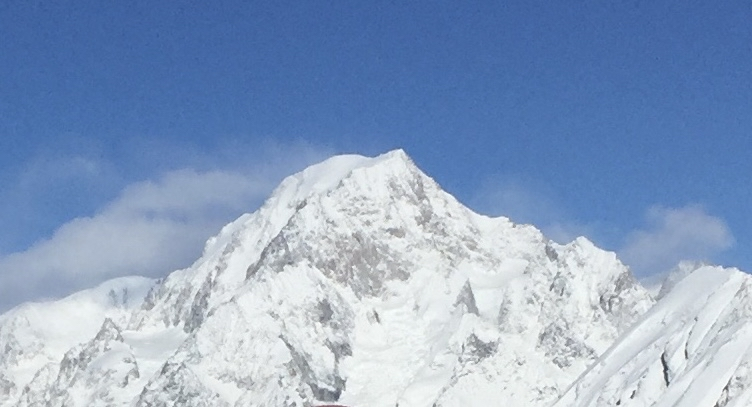
\includegraphics[width=4cm]
         {montblanc}};
      \node[text=white,
           font=\tiny\sffamily]
        at ([yshift=2mm]beartummy)
        {{Mont Blanc}};
     }]
   \end{scope}
 \end{tcblisting}

 \section{The brains behind \bearwearlogo{}}
 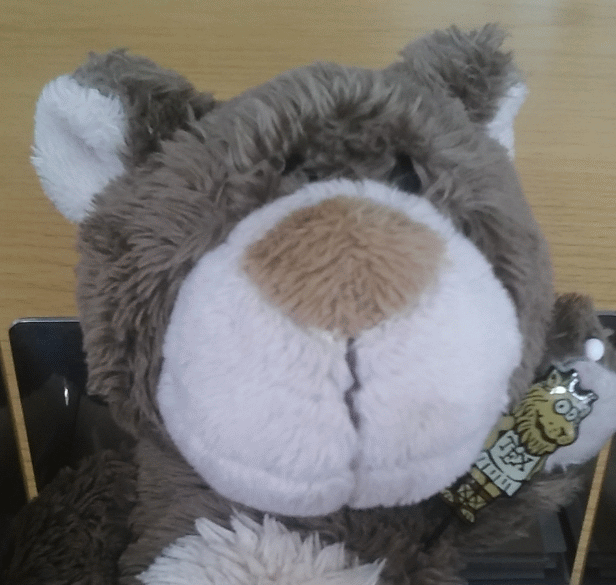
\includegraphics[width=3cm]{baer}
 \begin{description}
 \item[Ulrike]
  Bär, your decision to create \bearwearlogo{} has come as a surprise to many. Did you expect this?
  \item[Bär] Quite true, Ulrike. I am better known as an outdoor type
  and the fashionistas didn't reckon with me at all.
 \item[Ulrike] So, why did you take this step?
 \item[Bär] There were quite a few reasons -- most importantly
 my deeply felt desire to bring more justice to the world.
 Look at the wonderful world of \TikZ ducks fashion, and even Marmots have come
 far in the area of refinement. Why should \TikZ bears be left behind?
 \item[Ulrike] You are also concerned with the more momentous issues of our day.
 \item[Bär] Correct! My fashion line is the first ever to have practically
 no negative influence on our environment. Manufacture and transportation
 are ecologically neutral. In fact it's the first time in the
 history of world economy that goods are produced without
 the use of raw materials.
 \item[Ulrike] You claim that \bearwearlogo{} will have a global impact.
 \item[Bär] Yes, the issue of globalization is one which has been interesting
  me for a long time. \bearwearlogo{} caters for the needs of \TikZ bears all
  over the world. There is the Longshirt Line for those who live near the poles,
  t-shirts for those in temperate regions and even a Muscle Shirt Line for the
  bears of Australia.
 \item[Ulrike] How about individuality?
 \item[Bär] I am particularly proud that \bearwearlogo{} enables every single
 bear to create his own personal shirt -- free of the dictates of the modern
 Brummells. He may use my suggestions but he need not do so.
 \item[Ulrike] Will you be seen wearing your own creations?
 \item[Bär] Well Ulrike, I am afraid this is not very likely.
 I have got this most beautiful fur and I'd hate to  cover it with artifical
 patterns -- no matter how ravishing.
 \item[Ulrike] One last question: what impulse got you moving towards
 \bearwearlogo{}?
 \item[Bär] The death of Karl Lagerfeld. Someone had to fill the void.
 \end{description}
%</docu>
